\documentclass{article}

\usepackage{amsmath}
\usepackage{amssymb}
\usepackage{parskip}
\usepackage{fullpage}
\usepackage{graphicx}
\usepackage{hyperref}

\hypersetup{
    colorlinks=true,
    linkcolor=black,
    urlcolor=blue,
    pdftitle={Paolo Bettelini - Diaries},
    pdfpagemode=FullScreen,
}

\title{Diaries}
\author{Paolo Bettelini}
\date{}

\begin{document}

\maketitle
\tableofcontents
\pagebreak

\section{Diaries}

\subsection{2022-12-13}

Work hours:\\
\textbf{08:20 - 11:15}: Setup and research

Today I setup the git repository with the initial files
(CLI tool, documentation, etc.).
I then spent the rest of the working
session researching the topic of the project.

The planning has yet to be done.
The goal for the next working session is to make the Gantt chart.

\subsection{2022-12-14}

Work hours:\\
\textbf{15:10 - 16:20}: Alpha matting test \\
\textbf{16:00 - 16:20}: Gantt chart

Today I started using the \texttt{opencv} library (The Rust wrapper).
I used the sample images (target and trimap) from \href{https://docs.opencv.org/4.x/dd/d0e/tutorial\_alphamat.html}{https://docs.opencv.org/4.x/dd/d0e/tutorial\_alphamat.html}.
The output is not correct, but it shows some matting to be applied.
\begin{figure}[h]
    \centering
    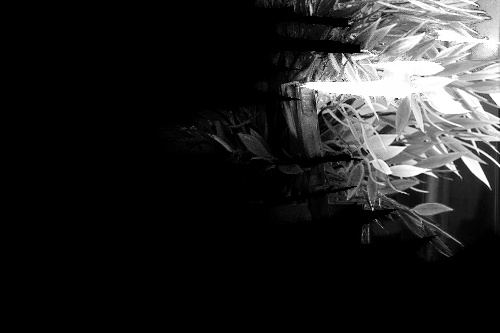
\includegraphics[width=0.75\textwidth]{res1}
\end{figure}

However, I noticed a small problem: when the input images are
wrong, instead of returning \texttt{Result(Err)} (as per Rust-philosophy),
it dumps the core.

I also started making the Gantt chart.

\pagebreak

\subsection{2022-12-15}

Work hours:\\
\textbf{08:20 - 09:50}: CLI executable \\
\textbf{10:20 - 11:20}: Gantt chart

Today I fixed the trimap matting. The trimap was being read using
\texttt{IMREAD\_COLOR} rather than \texttt{IMREAD\_GRAYSCALE}.
I then added the first CLI arguments to the executabl (target image,
trimap image, output image).
I need to find a solution to avoid the core dumps from \texttt{opencv}.

\begin{figure}[h]
    \centering
    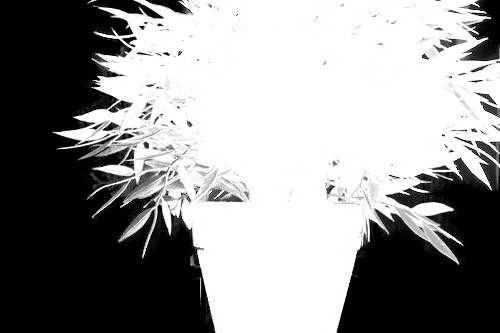
\includegraphics[width=0.75\textwidth]{res2}
\end{figure}

In the second half of the working session I completed the gantt chart

\subsection{2022-12-20}

Work hours:\\
\textbf{08:20 - 09:50}: OpenCV documentation \\
\textbf{10:20 - 11:20}: Documentation and requirements

In the first half of the working session I read
some documentation about OpenCV.
The goal is to be able to remove the background of an image
given its trimap.
In the second half I continued setting up the documentation
(requirements and layout).

\subsection{2022-12-21}

Work hours:\\
\textbf{15:05 - 15:30}: Documentation \\

Today I continued the analysis section.

\subsection{2022-12-22}

Work hours:\\
\textbf{08:20 - 09:50}: Background removal research \\
\textbf{10:05 - 10:30}: Read the review of my previous project documentation \\
\textbf{10:30 - 11:20}: GUI Research

Today I did not write any actual code, however, I did some research on which
technologies I will need to use. I realized that the background removal
cannot be done using \texttt{opencv}, but rather with another library.
Not much effort is necessary in order to finish the CLI tool, so I started
looking into the Rust GUI libraries. I also conitnued writing the requirements
in the analysis section.

The plan for the next working session is to finish the CLI tool.

\end{document}